\documentclass[12pt]{article}
\usepackage{geometry}
    \geometry{
    paperheight=40cm,
    paperwidth=21cm,
    left=30mm,
    top=20mm,
}
\usepackage{CJKutf8}
\usepackage{setspace}
\newcommand*{\ct}[1]{\linespread{1.5}\selectfont\begin{CJK*}{UTF8}{bsmi}#1\end{CJK*}}
\renewcommand\thesubsection{(\alph{subsection})}
\renewcommand\thesubsubsection{\roman{subsubsection}.}
\usepackage{titlesec}
\titleformat{\subsubsection}{\normalfont\bfseries}{\hspace*{30pt}\thesubsubsection}{10pt}{}
\usepackage{changepage}
\usepackage{calc}
\newenvironment{indentedSection}{
    \begin{adjustwidth}{30pt}{}
        \ignorespaces
    }{\end{adjustwidth}}
\usepackage{graphicx}
\usepackage{array}
\usepackage{multirow}
\usepackage{tikz}
\usetikzlibrary{shapes, positioning, calc, er}
\newcommand{\code}[1]{\ttfamily#1\rmfamily}
\usepackage{blindtext}
\usepackage{listings}
\usepackage{color}
\definecolor{dkgreen}{rgb}{0,0.6,0}
\definecolor{gray}{rgb}{0.5,0.5,0.5}
\definecolor{mauve}{rgb}{0.58,0,0.82}
\lstset{
    language=SQL,
    basicstyle={\ttfamily},
    belowskip=3mm,
    breakatwhitespace=true,
    breaklines=true,
    classoffset=0,
    columns=flexible,
    commentstyle=\color{dkgreen},
    framexleftmargin=0em,
    frameshape={}{}{}{}, %To remove to vertical lines on left, set `frameshape={}{}{}{}`
    keywordstyle=\color{blue},
    numbers=none, %If you want line numbers, set `numbers=left`
    numberstyle=\tiny\color{gray},
    showstringspaces=false,
    stringstyle=\color{mauve},
    xleftmargin =0em
}
\title{}
\author{}
\date{}
\begin{document}

\pagestyle{empty}

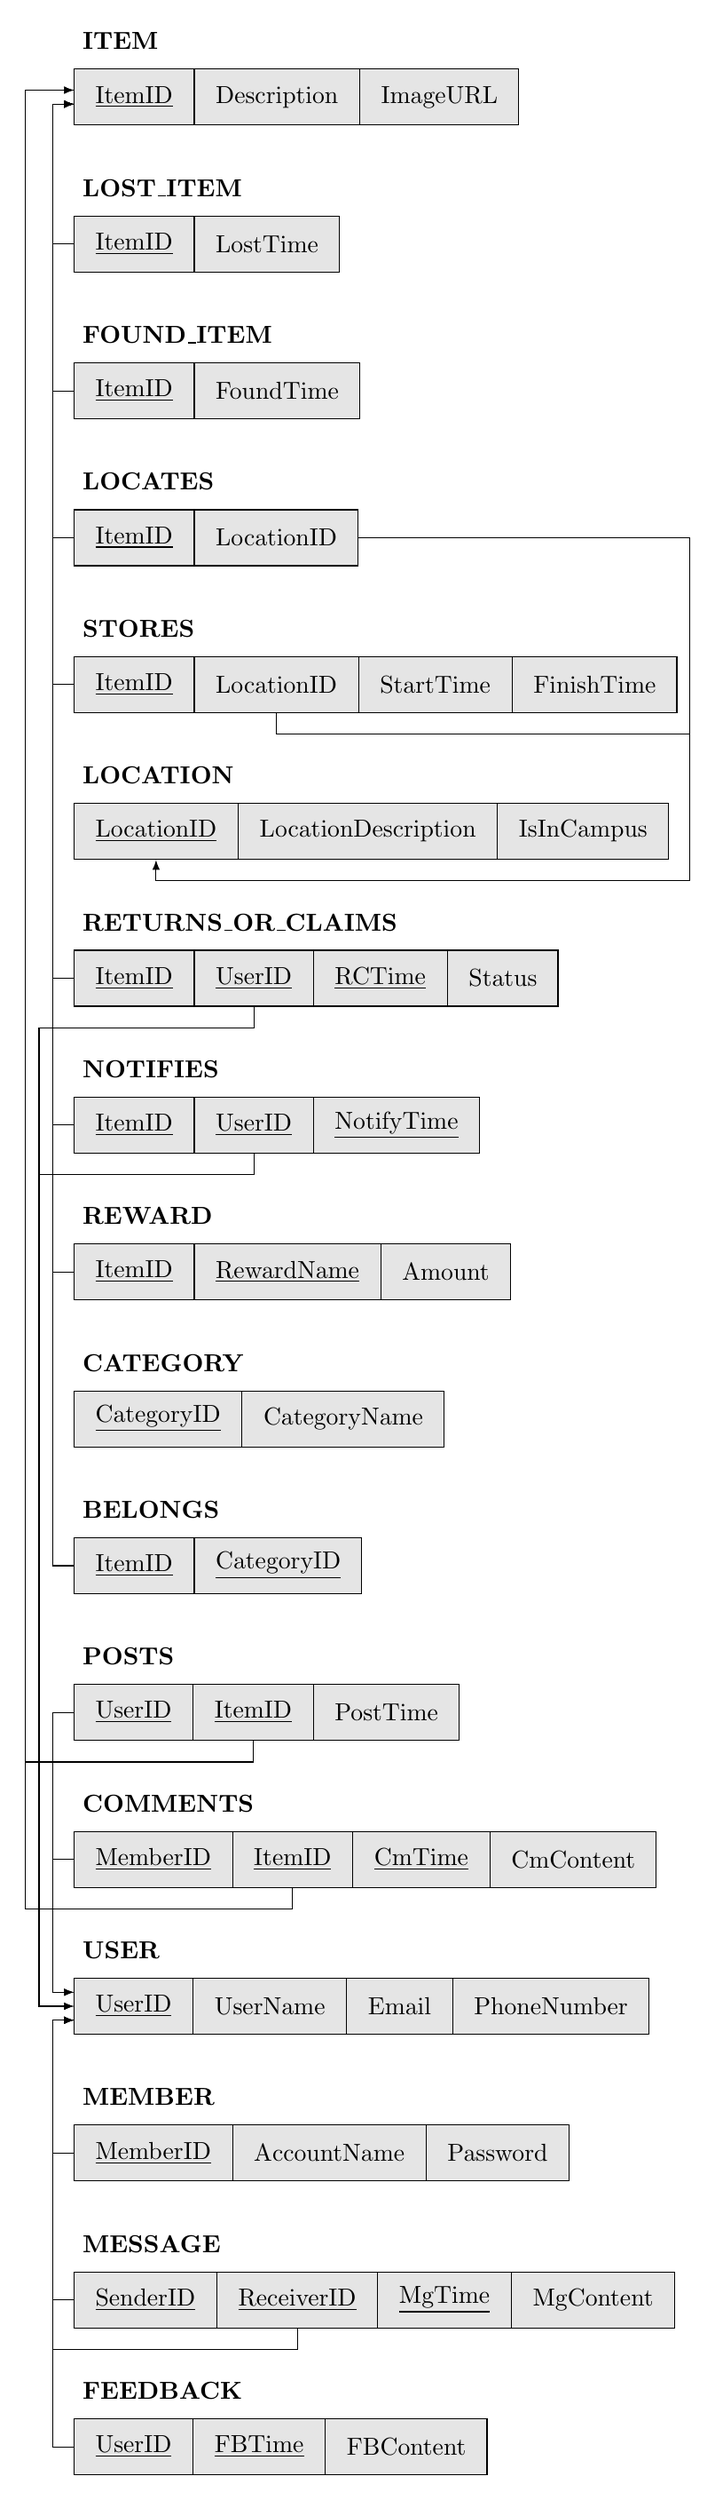
\begin{tikzpicture}[relation/.style={rectangle split, rectangle split parts=#1, rectangle split part align=center, draw, anchor=center, align=center, text centered, minimum height=.8cm, inner xsep=.3cm}]

\newcommand*{\nodelist}[2]{\node [relation=#1, rectangle split horizontal, rectangle split part fill={lightgray!40}, anchor=north west, below=.8cm of #2title.west, anchor=west] (#2)}

% RELATIONS

\node (itemtitle) {\textbf{ITEM}};

\nodelist{3}{item}
{\underline{ItemID}
\nodepart{two}   Description
\nodepart{three} ImageURL};

\node [below=1.3cm of item.west, anchor=west] (LItitle) {\textbf{LOST\_ITEM}};

\nodelist{2}{LI}               
{\underline{ItemID}
\nodepart{two}   LostTime};

\node [below=1.3cm of LI.west, anchor=west] (FItitle) {\textbf{FOUND\_ITEM}};

\nodelist{2}{FI}
{\underline{ItemID}
\nodepart{two}   FoundTime};

\node [below=1.3cm of FI.west, anchor=west] (lctitle) {\textbf{LOCATES}};

\nodelist{2}{lc}
{\underline{ItemID}
\nodepart{two}   LocationID};

\node [below=1.3cm of lc.west, anchor=west] (sttitle) {\textbf{STORES}};

\nodelist{4}{st}
{\underline{ItemID}
\nodepart{two}   LocationID
\nodepart{three} StartTime
\nodepart{four}  FinishTime};

\node [below=1.3cm of st.west, anchor=west] (lcttitle) {\textbf{LOCATION}};

\nodelist{3}{lct}
{\underline{LocationID}
\nodepart{two}   LocationDescription
\nodepart{three} IsInCampus};

\node [below=1.3cm of lct.west, anchor=west] (roctitle) {\textbf{RETURNS\_OR\_CLAIMS}};

\nodelist{4}{roc}
{\underline{ItemID}
\nodepart{two}   \underline{UserID}
\nodepart{three} \underline{RCTime}
\nodepart{four}  Status};

\node [below=1.3cm of roc.west, anchor=west] (nttitle) {\textbf{NOTIFIES}};

\nodelist{3}{nt}
{\underline{ItemID}
\nodepart{two}   \underline{UserID}
\nodepart{three} \underline{NotifyTime}};

\node [below=1.3cm of nt.west, anchor=west] (rwtitle) {\textbf{REWARD}};

\nodelist{3}{rw}
{\underline{ItemID}
\nodepart{two}   \underline{RewardName}
\nodepart{three} Amount};

\node [below=1.3cm of rw.west, anchor=west] (cttitle) {\textbf{CATEGORY}};

\nodelist{2}{ct}
{\underline{CategoryID}
\nodepart{two}   CategoryName};

\node [below=1.3cm of ct.west, anchor=west] (bltitle) {\textbf{BELONGS}};

\nodelist{2}{bl}
{\underline{ItemID}
\nodepart{two}   \underline{CategoryID}};

\node [below=1.3cm of bl.west, anchor=west] (ptitle) {\textbf{POSTS}};

\nodelist{3}{p}
{\underline{UserID}
\nodepart{two}   \underline{ItemID}
\nodepart{three}  PostTime};

\node [below=1.3cm of p.west, anchor=west] (cmtitle) {\textbf{COMMENTS}};

\nodelist{4}{cm}
{\underline{MemberID}
\nodepart{two}   \underline{ItemID}
\nodepart{three} \underline{CmTime}
\nodepart{four}  CmContent};

\node [below=1.3cm of cm.west, anchor=west] (usertitle) {\textbf{USER}};

\nodelist{4}{user}
{\underline{UserID}
\nodepart{two}   UserName
\nodepart{three} Email
\nodepart{four}  PhoneNumber};

\node [below=1.3cm of user.west, anchor=west] (mbtitle) {\textbf{MEMBER}};

\nodelist{3}{mb}
{\underline{MemberID}
\nodepart{two}   AccountName
\nodepart{three} Password};
            
\node [below=1.3cm of mb.west, anchor=west] (msgtitle) {\textbf{MESSAGE}};

\nodelist{4}{msg}
{\underline{SenderID}
\nodepart{two}   \underline{ReceiverID}
\nodepart{three} \underline{MgTime}
\nodepart{four}  MgContent};

\node [below=1.3cm of msg.west, anchor=west] (fbtitle) {\textbf{FEEDBACK}};

\nodelist{3}{fb}
{\underline{UserID}
\nodepart{two}   \underline{FBTime}
\nodepart{three} FBContent};

% FOREIGN KEYS

\draw[-latex] (LI.one west) -- ++(-.3,0) |- ($(item.one west) + (0,-.1)$);
\draw[-latex] (FI.one west) -- ++(-.3,0) |- ($(item.one west) + (0,-.1)$);
\draw[-latex] (lc.one west) -- ++(-.3,0) |- ($(item.one west) + (0,-.1)$);
\draw[-latex] (st.one west) -- ++(-.3,0) |- ($(item.one west) + (0,-.1)$);
\draw[-latex] (roc.one west) -- ++(-.3,0) |- ($(item.one west) + (0,-.1)$);
\draw[-latex] (nt.one west) -- ++(-.3,0) |- ($(item.one west) + (0,-.1)$);
\draw[-latex] (rw.one west) -- ++(-.3,0) |- ($(item.one west) + (0,-.1)$);
\draw[-latex] (bl.one west) -- ++(-.3,0) |- ($(item.one west) + (0,-.1)$);
\draw[-latex] (p.two south) -- ++(0,-.3) -| ($(item.one west) + (-.7,.1)$) -- ($(item.one west) + (0,.1)$);
\draw[-latex] (cm.two south) -- ++(0,-.3) -| ($(item.one west) + (-.7,.1)$) -- ($(item.one west) + (0,.1)$);
\draw[latex-] (lct.one south) -- ++(0,-.3) -| ($(lct.three east) + (.3,0)$) |- (lc.two east);
\draw         ($(lct.three east) + (.3,0)$) |- ($(st.two south) + (0,-.3)$) -- ++(0,.3);
\draw[latex-] ($(user.one west) + (0,-.2)$) -- ++(-.3,0) |- (mb.one west);
\draw[latex-] ($(user.one west) + (0,-.2)$) -- ++(-.3,0) |- (msg.one west);
\draw[latex-] ($(user.one west) + (0,-.2)$) -- ++(-.3,0) |- ($(msg.two south) + (0,-.3)$) -- (msg.two south);
\draw[latex-] ($(user.one west) + (0,-.2)$) -- ++(-.3,0) |- (fb.one west);
\draw[latex-] ($(user.one west) + (0,.2)$) -- ++(-.3,0) |- (cm.one west);
\draw[latex-] ($(user.one west) + (0,.2)$) -- ++(-.3,0) |- (p.one west);
\draw[latex-] (user.one west) -- ++(-.5,0) |- ($(nt.two south) + (0,-.3)$) -- ++(0,.3);
\draw[latex-] (user.one west) -- ++(-.5,0) |- ($(roc.two south) + (0,-.3)$) -- ++(0,.3);
            
\end{tikzpicture}

% \begin{tikzpicture}[node distance=2cm]
% \tikzstyle{every entity}=[draw=black,fill=lightgray!40,inner xsep=.4cm]
% \tikzstyle{every relationship}=[draw=black,fill=lightgray!40,inner xsep=.4cm]
% \tikzstyle{every pin edge}=[draw]

% \node[entity,pin={[attribute,yshift=10pt]120:\underline{SID}}]
%     (student)        at(0,0)               {STUDENT};
% \node[entity,pin={[attribute,yshift=10pt]70:\underline{Semester}},pin={[attribute]-100:Large\_Num},pin={[attribute]-50:Small\_Num}] 
%     (avc)            at(12,0)              {AVAILABLE\_CLOSET};
% \node[relationship,pin={[attribute]40:Status},pin={[attribute]140:Large\_Num},pin={[attribute]90:Small\_Num}] 
%     (apply)          at(5.5,2)               {APPLIES};
% \node[relationship,pin={[attribute]-120:Large\_Num},pin={[attribute]-60:Small\_Num}] 
%     (use)            at(5.5,-2)              {USES};
% \draw (student) -- node[pos=.5,xshift=-8pt,yshift=8pt]{(0,\,1)} (apply);
% \draw (avc) -- node[pos=.5,xshift=7pt,yshift=8pt]{(0,\,1)} (apply);
% \draw (student) -- node[pos=.5,xshift=4pt,yshift=9pt]{(0,\,1)} (use);
% \draw (avc) -- node[pos=.5,xshift=-4pt,yshift=8pt]{(0,\,1)} (use);
% \end{tikzpicture}
% \subsection{}
% \vspace*{.5cm}
% \begin{tikzpicture}[relation/.style={rectangle split, rectangle split parts=#1, rectangle split part align=center, draw, anchor=center, align=center, text centered, minimum height=.8cm, inner xsep=.3cm}]

% \hspace*{15pt}
% \newcommand*{\nodelist}[2]{\node [relation=#1, rectangle split horizontal, rectangle split part fill={lightgray!40}, anchor=north west, below=.8cm of #2title.west, anchor=west] (#2)}

% % RELATIONS

% \node (studenttitle) {\textbf{STUDENT}};

% \nodelist{1}{student}
% {\underline{SID}};

% \node [below=1.3cm of student.west, anchor=west] (applytitle) {\textbf{APPLIES}};

% \nodelist{5}{apply}               
% {\nodepart{one}\raisebox{-2.5pt}{\underline{SID}}
% \nodepart{two}   Large\_Num
% \nodepart{three} Small\_Num
% \nodepart{four}  Status
% \nodepart{five}  \underline{Semester}};

% \node [below=1.3cm of apply.west, anchor=west] (usetitle) {\textbf{USES}};

% \nodelist{4}{use}
% {\underline{SID}
% \nodepart{two}   Large\_Num
% \nodepart{three} Small\_Num
% \nodepart{four}  \underline{Semester}};

% \node [below=1.3cm of use.west, anchor=west] (avctitle) {\textbf{AVAILABLE\_CLOSET}};

% \nodelist{3}{avc}
% {\underline{Semester}
% \nodepart{two}   Large\_Num
% \nodepart{three} Small\_Num};

% % FOREIGN KEYS

% \draw[-latex] (apply.one west) -- ++(-.5,0) |- (student.one west);
% \draw[-latex] (use.one west) -- ++(-.5,0) |- (student.one west);
% \draw[-latex] (apply.five south) |- ($(avc.one south) + (0,-.5)$) -- (avc.one south);
% \draw (use.four east) -| (apply.five south);
            
% \end{tikzpicture}

\end{document}